% Slides for Seminar on Function-Space Variational Inference in the context of Implicit Processes.
% November 30, 2022

% Compile using XeLatex

\documentclass[10pt, aspectratio=149]{beamer}

\usetheme[progressbar=frametitle]{metropolis}
\setbeamertemplate{section in toc}[sections numbered]
\setbeamertemplate{subsection in toc}[subsections numbered]


% IMPORTS and PACKAGES
\usepackage{appendixnumberbeamer}

\usepackage{booktabs}
\usepackage[scale=2]{ccicons}

\usepackage{amsthm}
\DeclareMathOperator*{\argmax}{arg\,max}
\DeclareMathOperator*{\argmin}{arg\,min}
\usepackage{pgfplots}
\usepgfplotslibrary{dateplot}
\usepackage{multirow}
\setbeamercovered{transparent}
\usepackage{xspace}
\newcommand{\themename}{\textbf{\textsc{metropolis}}\xspace}
\usepackage{mathtools}
\usefonttheme{professionalfonts} % required for mathspec
\usepackage{mathspec}
\setsansfont[BoldFont={Fira Sans}]{Fira Sans Light}
\usepackage{cancel}
\usepackage{bm}

% SEMINAR INFORMATION

\title{Function-Space Variational Inference in the context of Implicit Processes}
\subtitle{Machine Learning Group}
\date{\today}
\author{Luis Antonio Ortega Andrés}
\institute{Autonomous University of Madrid}

% Change Metropolis progress bar width
\makeatletter
\setlength{\metropolis@titleseparator@linewidth}{1pt}
\setlength{\metropolis@progressonsectionpage@linewidth}{1pt}
\setlength{\metropolis@progressinheadfoot@linewidth}{1pt}
\makeatother


% Change separation in TOC
\makeatletter
\patchcmd{\beamer@sectionintoc}
  {\vfill}
  {\vskip 1.8\itemsep}
  {}
  {}
\makeatother  




% DOCUMENT

\begin{document}

\maketitle

\begin{frame}{Motivation}
    \begin{center}
    	\includegraphics<1>[width=0.7\textwidth]{imgs/intro_1.pdf}\includegraphics<2>[width=0.7\textwidth]{imgs/intro_2.pdf}\includegraphics<3>[width=0.7\textwidth]{imgs/intro_3.pdf}\includegraphics<4>[width=0.7\textwidth]{imgs/intro_4.pdf}\includegraphics<5->[width=0.7\textwidth]{imgs/intro_5.pdf}
    
    \only<1>{\textbf{Objective}: Make predictions over unknown points.}
    \only<2>{\textbf{Procedure}: Learn a function that explain the visible data.}
    \only<3>{\textbf{Outcome}: The function can be used to predict.}
    \only<4>{\textbf{Question}: How confident is the prediction?}
    \only<5->{\textbf{Answer}: Bayesian approach.}
    \end{center}
\end{frame}


\begin{frame}{Overview}
    \begin{columns}[t]
        \begin{column}{.5\textwidth}
            \tableofcontents[ 
            sections={1-4}
            ] 
        \end{column}
        \begin{column}{.5\textwidth}
            \tableofcontents[sections={5-7}]
        \end{column}
    \end{columns}
\end{frame}


\section{Bayesian Supervised Learning}

 \begin{frame}{Bayesian Supervised Learning}
    \begin{overprint}
        \onslide<1> 
            \vspace{0.5cm}
            \textbf{Objective}: Learn an unknown function \(f:\mathbb R^D \to \mathbb R^M\) given a set of observations \(\mathbf X = (\mathbf x_1,\dots,\mathbf x_N) \subset \mathbb R^D, \mathbf y = (y_1,\dots,y_N) \subset \mathbb R^M\).\\
        
            \textbf{Approach. }Consider a set of latent random variables \(\mathbf z\) that model the generation of the dataset \(P(\mathbf y | \mathbf X, \mathbf z)\).
      \onslide<2> 
        \vspace{0.5cm}
          \textbf{Problem. }Prediction requires the posterior \(P(\mathbf z | \mathbf X, \mathbf y)\):
            \[
                P(y_\star | \mathbf x_\star, \mathbf X, \mathbf y) = \int P(y_\star | \mathbf x_\star, \mathbf z)P(\mathbf z | \mathbf X, \mathbf y)\, d\mathbf z\,,
            \]
            which is usually intractable due to the integral
            \[
                P(\mathbf z | \mathbf X, \mathbf y) = \frac{P(\mathbf y, \mathbf{z}|\mathbf X)}{\int P(\mathbf y, \mathbf{z}|\mathbf X) \, d\mathbf z}\,.
            \]
    \end{overprint}
    
    \begin{overprint}
        \vspace{0.3cm}
        \hspace{2.5cm} Prior \hspace{1.7cm} Likelihood  \hspace{1.4cm} Posterior
        \begin{center}
        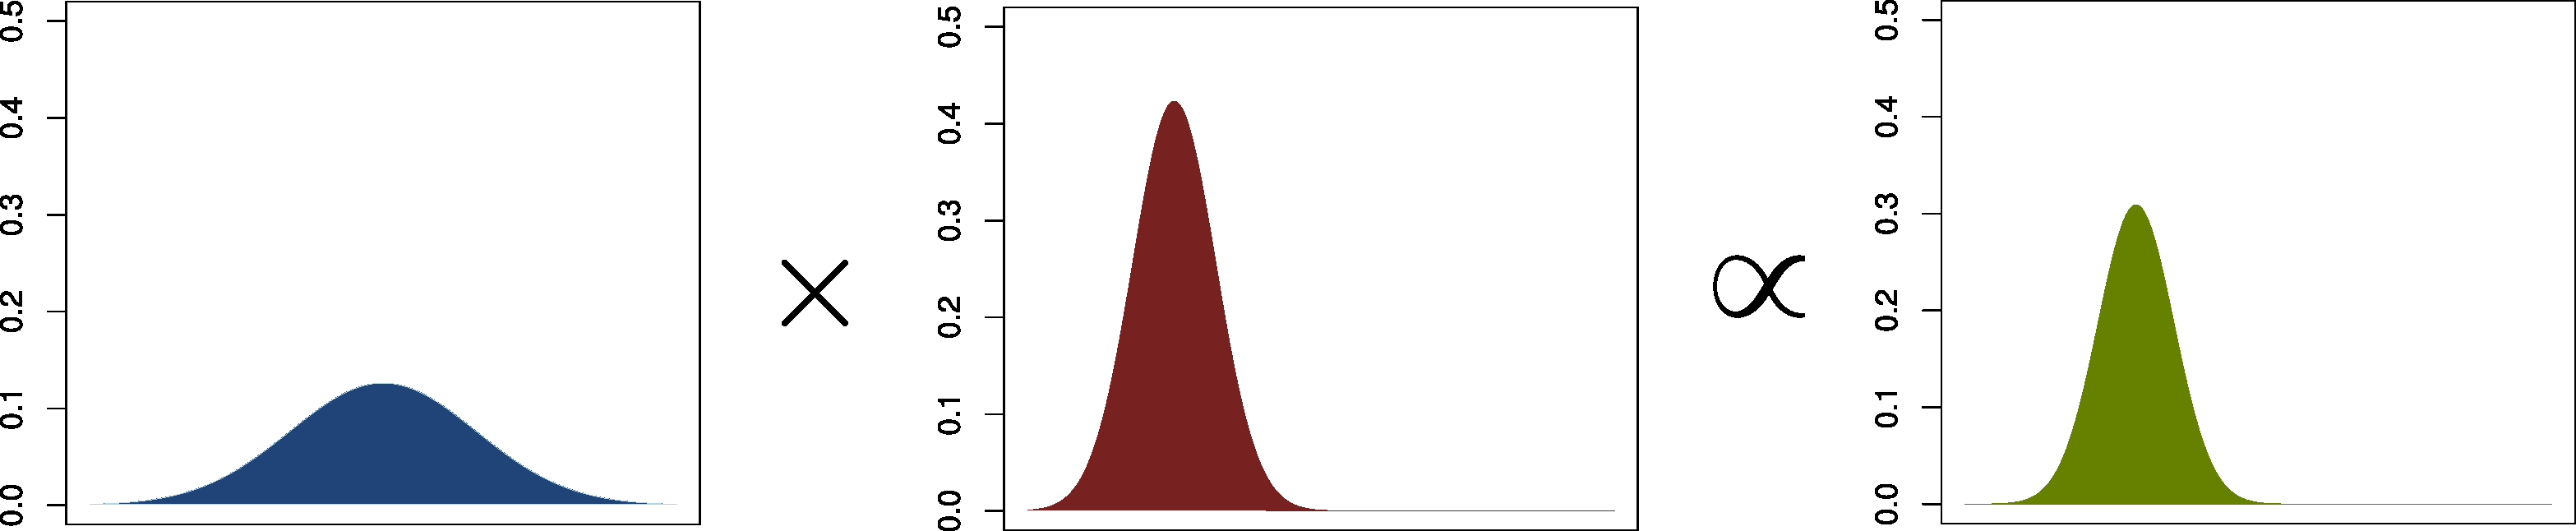
\includegraphics[width=0.7\textwidth]{imgs/bayes_rule.pdf}
        \end{center}
    \end{overprint}
\end{frame}

\section{Variational Inference}

  \begin{frame}{Variational Inference}
     \textbf{Idea.} Approximate the posterior \(P(\mathbf z | \mathbf X, \mathbf y)\) with a \textbf{\alert{simpler distribution}} \(Q(\mathbf z)\) and ensure that
     \(
        KL\Big(Q(\mathbf z)\mid  P(\mathbf z | \mathbf X, \mathbf y)  \Big)
     \)
     is close to \(0\).

     Formally,
    \begin{align*}
    \only<1>{
        Q^\star(\mathbf z) &= \argmin_{Q \in \mathcal{Q}}\, KL\Big(Q(\mathbf z)  \mid P(\mathbf z | \mathbf X, \mathbf y)\Big)\\
        &= \argmax_{Q \in \mathcal{Q}} \,\mathbb{E}_{Q(\mathbf z)}\Big[ \log P(\mathbf y | \mathbf X, \mathbf z) \Big] - KL\Big(Q(\mathbf z) \mid P(\mathbf z) \Big)\,.\\
    }
    \only<2>{
        Q^\star(\mathbf z) &= \argmin_{Q \in \mathcal{Q}}\, KL\Big(Q(\mathbf z)  \mid P(\mathbf z | \mathbf X, \mathbf y)\Big)\\
        &= \argmax_{Q \in \mathcal{Q}} \,\underbrace{\mathbb{E}_{Q(\mathbf z)}\Big[ \log P(\mathbf y | \mathbf X, \mathbf z) \Big] - KL\Big(Q(\mathbf z) \mid P(\mathbf z) \Big)}_{\text{\textbf{ELBO}}}\,.\\
    }
    \only<3>{
        Q^\star(\mathbf z) &= \argmin_{Q \in \mathcal{Q}}\, KL\Big(Q(\mathbf z)  \mid P(\mathbf z | \mathbf X, \mathbf y)\Big)\\
        &= \argmax_{Q \in \mathcal{Q}} \,\underbrace{\mathbb{E}_{Q(\mathbf z)}\Big[ \log P(\mathbf y | \mathbf X, \mathbf z) \Big]}_{\text{\textbf{Data Fitting term}}} - \underbrace{KL\Big(Q(\mathbf z) \mid P(\mathbf z) \Big)}_{\text{\textbf{Regularizer}}}\,.\\
    }
    \end{align*}
 \end{frame}

\section{Gaussian Processes}

    \begin{frame}{Gaussian Processes}
        A \textbf{\alert{Gaussian process}} (GP) is a collection of random variables \( f(\cdot) \) such that any finite collection \( \mathbf f = \{f(\mathbf x_1), f(\mathbf x_2), \dots, f(\mathbf x_N) \} \) follows a Gaussian distribution
        \[
            \mathbf f = f(\mathbf X) = \Big(f(\mathbf x_1),\dots,f(\mathbf x_N)\Big) \sim \mathcal{N}\Big(m(\mathbf X), \kappa(\mathbf X, \mathbf X)\Big)\,.
        \]
        Gaussian processes place a \textbf{probability distribution over functions}.

        Usually, 
        \[
            m(\mathbf x) = 0\quad \text{and} \quad            \kappa(\mathbf x_1, \mathbf x_2) = \sigma^2 \exp \left(- \frac{\|\mathbf x_1 - \mathbf x_2 \|_2^2}{2l^2} \right)\,.
        \]

    \end{frame}
    \begin{frame}

        \textbf{Hypothesis: } The unknown function \(f\) is a (noisy) sample from a Gaussian process.

        \begin{figure}
            \centering
            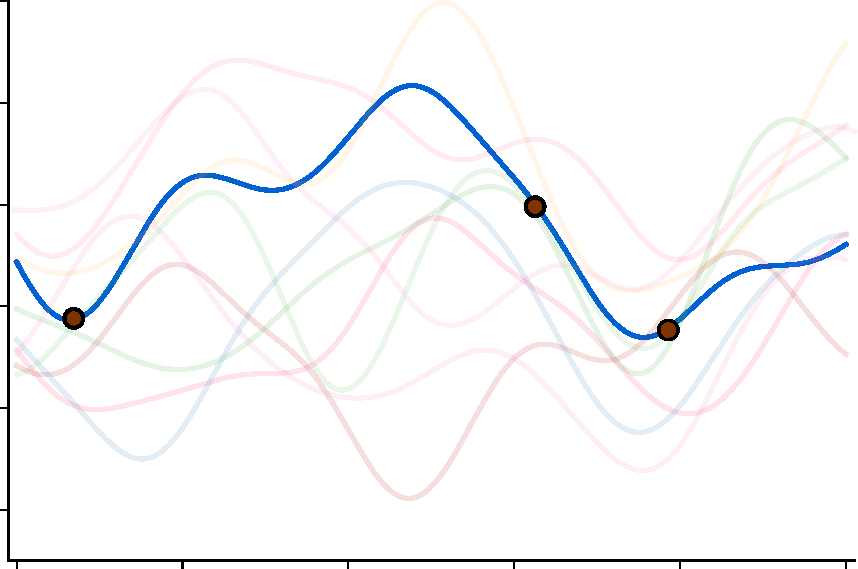
\includegraphics[width=0.7\textwidth]{imgs/GP_hypothesis.pdf}
        \end{figure}
    \end{frame}


    \begin{frame}
        For a regression problem, using,
        \begin{itemize}
            \item the Gaussian process prior over functions, \[ P(\mathbf f) = \mathcal{N}\Big(m(\mathbf X), \kappa(\mathbf X, \mathbf X)\Big)\,,\]
            \item a suitable likelihood  \[P(\mathbf y| \mathbf f) = \mathcal{N}(\mathbf f, \sigma^2 \mathbf I)\,.\]
        \end{itemize}
        Predictive distribution is computable in closed form
        \[
            P\big(f(\mathbf x^\star)|\mathbf y, \mathbf X\big) = \mathcal{N}( \mathbf \mu^\star, \mathbf \Sigma^\star)\,,
        \]
        with
        \begin{align*}
             \mathbf \mu^\star &= m(\mathbf x^\star) + \kappa(\mathbf x^\star, \mathbf X)(\kappa(\mathbf X, \mathbf X) + \sigma^2\mathbf I)^{-1}(\mathbf y - m(\mathbf X))\,,\\
             \mathbf \Sigma^\star &= \kappa(\mathbf x^\star, \mathbf x^\star) - \kappa(\mathbf x^\star, \mathbf X)(\kappa(\mathbf X, \mathbf X) + \sigma^2\mathbf I)^{-1}\kappa(\mathbf X, \mathbf x^\star)\,.
        \end{align*}
    \end{frame}

    \begin{frame}
            \begin{align*}
             \mathbf \mu^\star &= m(\mathbf x^\star) + \kappa(\mathbf x^\star, \mathbf X)(\kappa(\mathbf X, \mathbf X) + \sigma^2\mathbf I)^{-1}(\mathbf y - m(\mathbf X))\,,\\
             \mathbf \Sigma^\star &= \kappa(\mathbf x^\star, \mathbf x^\star) - \kappa(\mathbf x^\star, \mathbf X)(\kappa(\mathbf X, \mathbf X) + \sigma^2\mathbf I)^{-1}\kappa(\mathbf X, \mathbf x^\star)\,.
        \end{align*}
        \begin{figure}
            \centering
            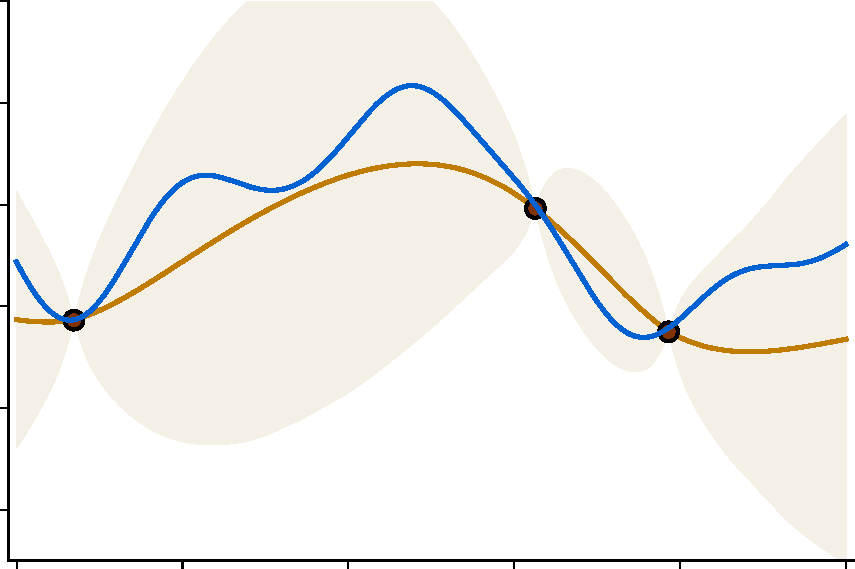
\includegraphics[width=0.75\textwidth]{imgs/GP_pred.pdf}
        \end{figure}
    \end{frame}

    \begin{frame}
        
        Hyper-parameters (kernel and likelihood) can be \textbf{optimized} using the marginal log likelihood:
        \[
            \log P(\mathbf y) = -\frac{1}{2}\mathbf y^T(\mathbf K + \sigma^2 \mathbf I)^{-1}\mathbf y - \frac{1}{2}\log \det (\mathbf K + \sigma^2 \mathbf I) - \frac{N}{2}\log 2\pi\,,
        \]
        with \(\mathbf K = \kappa(\mathbf X, \mathbf X)\).
        
        \vspace{1cm}
        
        \onslide<2->
        \textbf{\alert{Limitation.}} Requires the computation of \((\mathbf K + \sigma^2 \mathbf I)^{-1}\) which is \(\mathcal O(N^3)\).\\
        \textbf{\alert{Limitation.}} Mini-batches cannot be used for optimization.
    \end{frame}

    \subsection{Sparse Gaussian Processes}
    \begin{frame}{Sparse Gaussian Processes}
        \only<1>{
            Initialize a set of \textbf{\alert{inducing locations}}  \(\mathbf Z\) with \(|\mathbf Z| < |\mathbf X|\). For example \(\mathbf Z\) can be the centers of applying KMeans to \(\mathbf X\).
        }
        \only<2>{
            Set a variational distribution over the \textbf{\alert{inducing points}} \( \bm u = f(\mathbf Z)\), typically, \(Q(\bm u) = \mathcal{N}(\bm m, \bm S)\).
        }
        \only<3>{
            The approximated posterior predictive distribution is,
            \[
             Q( f(\mathbf x_\star)) = \int_{\bm u} P( f(\mathbf x_\star)| \bm u)Q(\bm u) = \mathcal{N}(\bm \mu, \bm \Sigma)
            \]
            is Gaussian and suitable for making predictions.
        }
            \begin{center}
                \includegraphics<1>[width=.7\linewidth]{imgs/GP_inducing_1.pdf}
                \includegraphics<2>[width=.7\linewidth]{imgs/GP_inducing_2.pdf}
                \includegraphics<3>[width=.6\linewidth]{imgs/GP_inducing_3.pdf}
            \end{center}
    \end{frame}
    \begin{frame}
            Minimize the ELBO to optimize \(Q(\bm u, \mathbf f)\), with \(\mathbf f = (f(\mathbf x_1),  \dots, f(\mathbf x_N))\),
            \begin{align*}
                Q^\star(\bm u,  \mathbf f) &= \argmin_{Q \in \mathcal{Q}}\, KL\Big(Q(\bm u,  \mathbf f)  \mid P(\bm u,  \mathbf f | \mathbf X, \mathbf y)\Big)\\
                &= \argmax_{Q \in \mathcal{Q}} \,\mathbb{E}_{Q( \mathbf f)}\Big[ \log P(\mathbf y | \mathbf X,  \mathbf f) \Big] - KL\Big(Q(\bm u) \mid P(\bm u) \Big)\,.\\
            \end{align*}    
            where 
            \begin{enumerate}
                \item \(P(\bm u)\) is given by the Gaussian Process distribution evaluated at \(\mathbf Z\).
                \item The Kullback-Leibler divergence is between Gaussian distributions.
                \item The data-fitting term can be computed for Gaussian likelihoods or approximated by quadrature.
            \end{enumerate}
    \end{frame}

\section{Implicit Processes}

    \begin{frame}{Implicit Processes}
        \textbf{\alert{Motivation}}: Gaussian processes are limited by the parametric kernel family.

        \begin{itemize}
            \item Square exponential kernel: \(\kappa(\mathbf x_1, \mathbf x_2) = \sigma^2 \exp \left(- \frac{\|\mathbf x_1 - \mathbf x_2 \|_2^2}{2l^2} \right) \).
            \item Linear kernel: \(\kappa(\mathbf x_1, \mathbf x_2) = a \mathbf x_1^T \mathbf x_2 + b\).
        \end{itemize}

        \begin{figure}
            \centering
            \begin{tabular}{cc}
              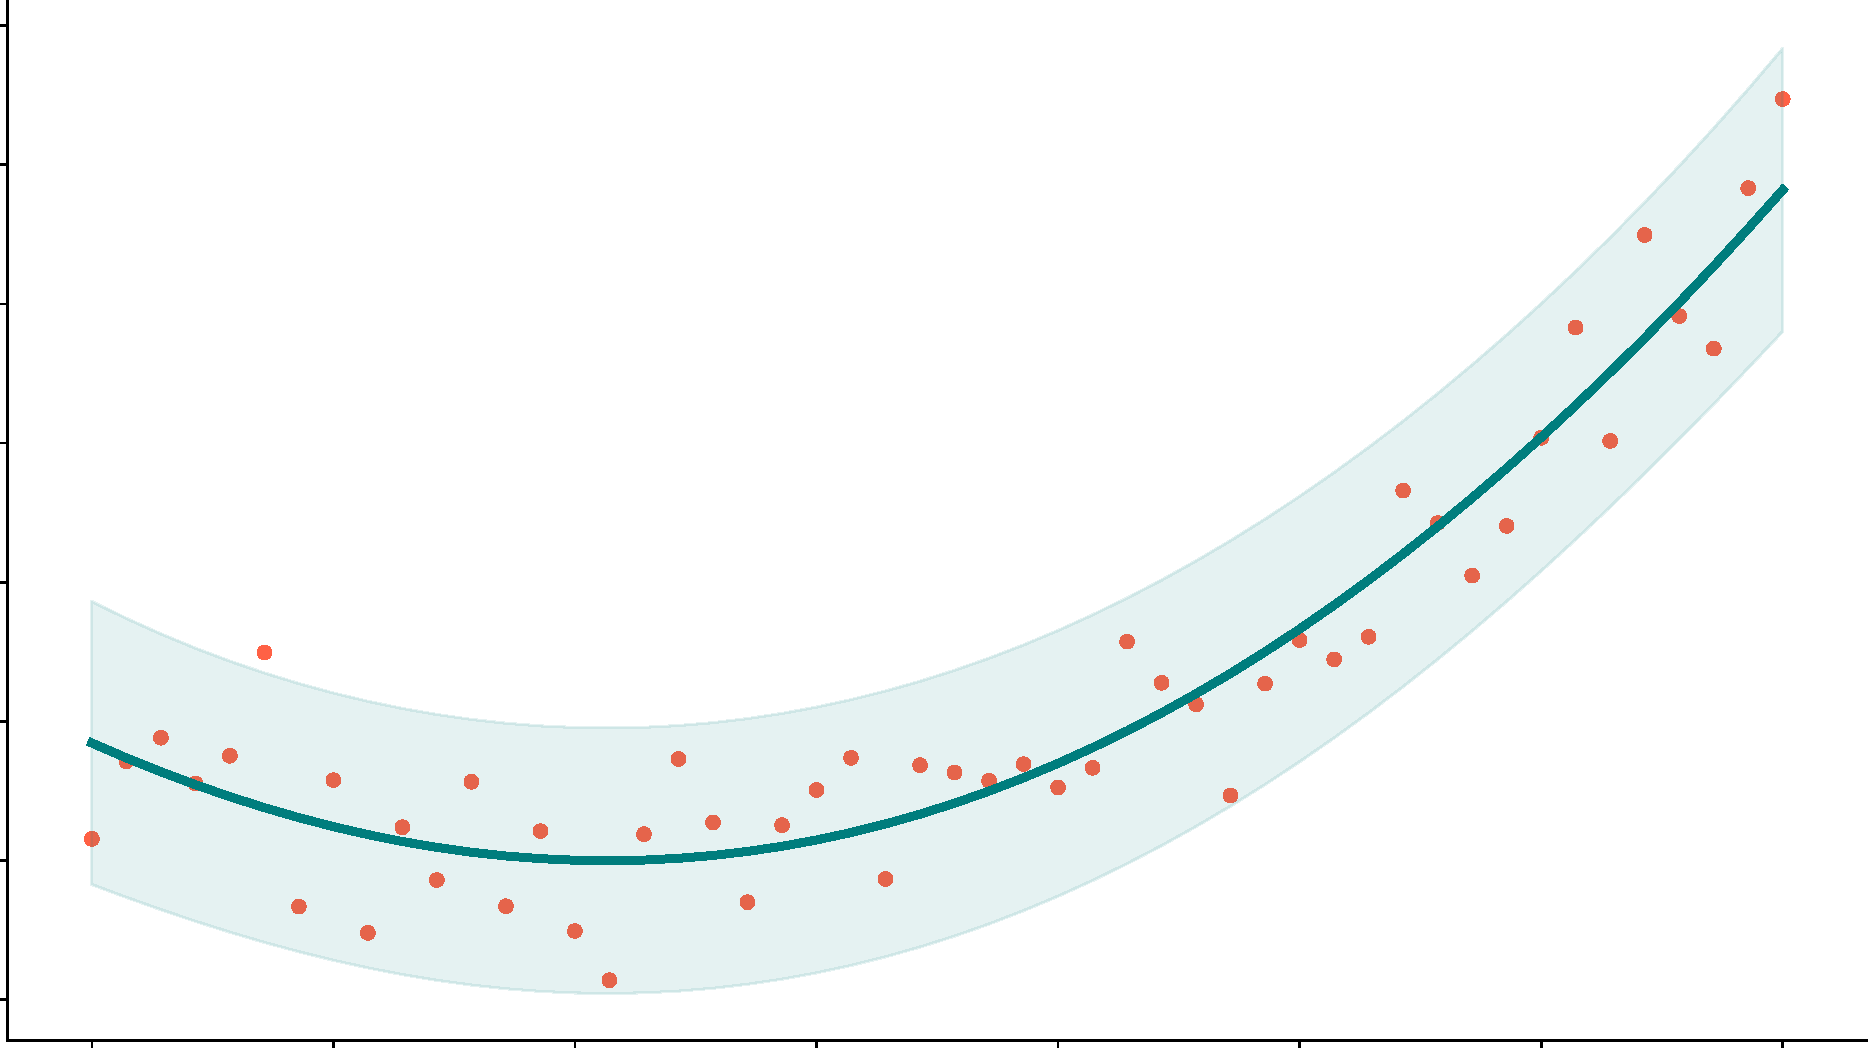
\includegraphics[width=.46\linewidth]{imgs/GP_RBF.pdf} &
              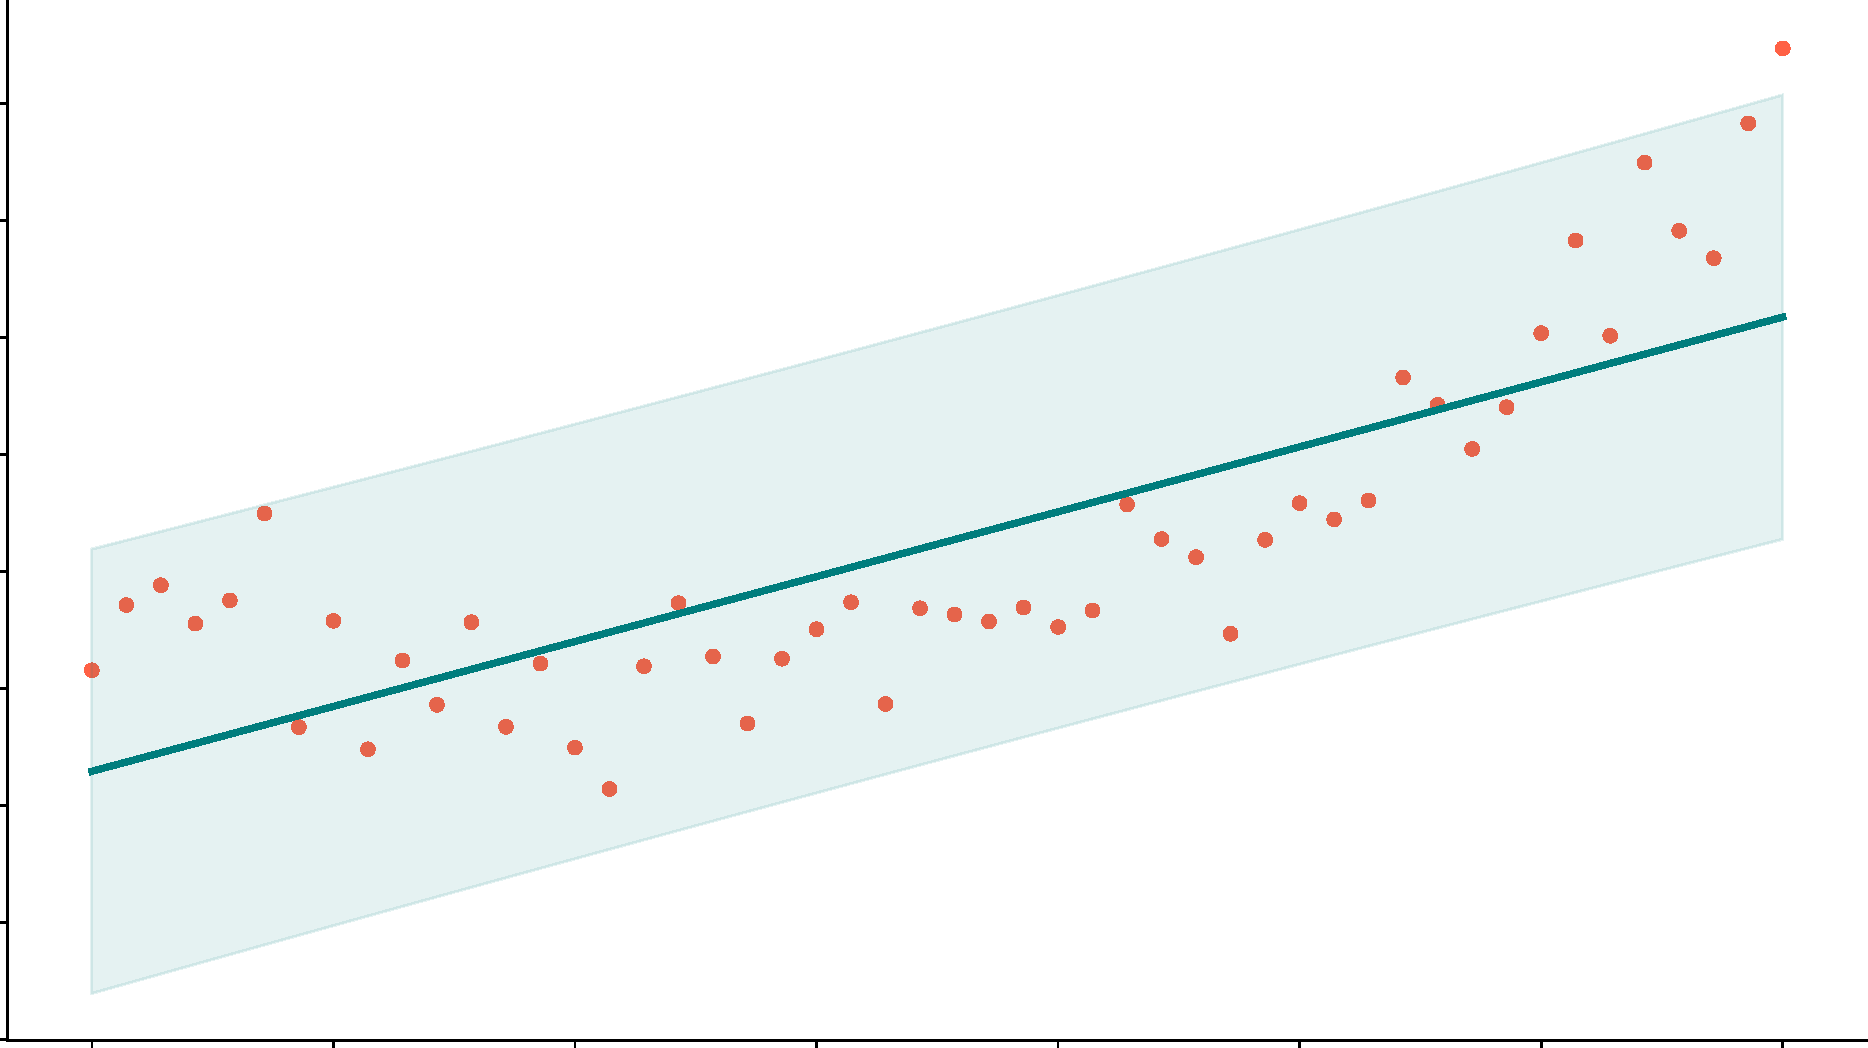
\includegraphics[width=.46\linewidth]{imgs/GP_DOT.pdf}
            \end{tabular}
        \end{figure}
        The Gaussian process prior over functions is \textbf{\alert{too restrictive}}.
    \end{frame}

    \begin{frame}
    \begin{overprint}
        An \textbf{\alert{implicit stochastic process}}\footnote{
Ma, C., Li, Y. \& Hernandez-Lobato, J.M.. (2019). Variational Implicit Processes.} (IP) is a collection of random variables \( f(\cdot) \) such that any finite collection \( \mathbf f = \{f(\mathbf x_1), f(\mathbf x_2), \dots, f(\mathbf x_N) \} \) is implicitly defined by the following generative process:
        \[
            \mathbf z \sim P_{\mathbf z}(\mathbf z) \quad \text{\emph{and}} \quad f(\mathbf x_n) = g_{\mathbf \theta}(\mathbf x_n, \mathbf z), \ \forall n =1, \dots, N\,.
        \]
        \end{overprint}
    \begin{overprint}
    \onslide*<2>{
        \textbf{Gaussian process}
            \[
                \mathbf z \sim \mathcal{N}(\bm 0, \bm I) \quad \text{\emph{and}} \quad f(\mathbf x_n) = \bm L(\mathbf x_n)^T\mathbf z, \ \forall n =1, \dots, N\,.
            \]
    }
    \onslide*<3>{
        \begin{minipage}{0.4\textwidth}
            \textbf{Bayesian Neural Networks}. 
            \[
                (\mathbf z_1, \mathbf z_2) \sim \mathcal{N}(\bm 0, \bm I)
            \]
            \[
                \bm \theta = (\bm \mu_1, \bm \mu_2, \bm \sigma_1, \bm \sigma_2)
            \]
            \[
                \bm h = r((\bm \mu_1 + \bm \sigma_1 \mathbf z_1)^T\mathbf{x}_n)\,.
            \]
            \[
                g_{\mathbf \theta}(\mathbf x_n, \mathbf z) = (\bm \mu_2 + \bm \sigma_2 \mathbf z_2)^T \bm h
            \]
        \end{minipage}%
        \begin{minipage}{0.6\textwidth}
        \begin{figure}
            \centering
            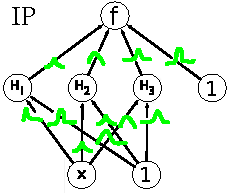
\includegraphics[width=0.6\textwidth]{imgs/BNN.pdf}
        \end{figure}
        \end{minipage}
    }
    \end{overprint}
    \end{frame}



    \begin{frame}{Variational Inference on Implicit Processes}
    \textbf{Problem statement:}
        \begin{enumerate}
            \item The unknown target function \textbf{is a sample from an IP}, that is, an implicit distribution over stochastic processes \(P(f(\cdot))\).
            \item Given the set of observations \((\mathbf X, \mathbf y)\), we aim to approximate the posterior distribution over functions \(P(f(\cdot)| \mathbf X, \mathbf y)\).
        \end{enumerate}
        \textbf{Approach}: Use variational inference over the function-space distribution \(Q(f(\cdot))\).
        \[
        \begin{aligned}
        Q^\star(f(\cdot))&= \argmin_{Q \in \mathcal{Q}}\, KL\Big(Q(f(\cdot))  \mid P( f(\cdot) | \mathbf X, \mathbf y)\Big)\\
        &= \argmax_{Q \in \mathcal{Q}} \,\mathbb{E}_{Q(f)}\Big[ \log P(\mathbf y | \mathbf X, f(\mathbf X)) \Big] - KL\Big(Q(f(\cdot)) \mid P(f(\cdot)) \Big)\,.
        \end{aligned}
        \]
    \end{frame}
    \begin{frame}
        \textbf{Approach}: Use variational inference over the function-space distribution
        \[
            Q^\star(f(\cdot)) = \argmax_{Q \in \mathcal{Q}} \,\mathbb{E}_{Q(f)}\Big[ \log P(\mathbf y | \mathbf X, f(\mathbf X)) \Big] - KL\Big(Q(f(\cdot)) \mid P(f(\cdot)) \Big)\,.
        \]
        \textbf{Difficulties:}
        \begin{enumerate}
            \item The prior \(P(f(\cdot))\) lacks a closed form.
            \item The Kullback-Leibler divergence between stochastic processes is not well-defined.
            \item The variational distribution \(Q(f(\cdot))\) must allow to compute or approximate by samples the data-fitting term.
        \end{enumerate}
    \end{frame}

    \begin{frame}{Existing Approaches}
        \textbf{\alert{Variational Implicit Processes}}\footnote{
            Ma, C., Li, Y. \& Hernandez-Lobato, J.M.. (2019). Variational Implicit Processes.}: Approximates the distribution over functions using a \textbf{linear combination of samples}.\\
        \vspace{0.5cm}
        \textbf{\alert{Sparse Implicit Processes}}\footnote{
            Rodríguez-Santana, S., Zaldivar, B. \& Hernandez-Lobato, D.. (2022). Function-space Inference with Sparse Implicit Processes.}: Uses \textbf{inducing points} for scalability and approximates the KL using an \textbf{external discriminator} (a Neural Network).\\
        \vspace{0.5cm}
        \textbf{\alert{Linearized approximation}}\footnote{
            Rudner, T., Chen, Z., Whye Y. \& Gal, Y.. (2022). Tractable Function-Space Variational Inference in Bayesian Neural Networks.}: Approximates the distribution over functions using a \textbf{linearization} of the BNN over the parameters.
    \end{frame}

    \subsection{Variational Implicit Processes}
    \begin{frame}{Variational Implicit Processes}
        Approximate \(P(f(\cdot))\) with a GP \(P_{\mathcal{GP}}(f(\cdot))\) \textbf{based on samples} \(f_1(\cdot),\dots,f_S(\cdot)\).
        Let
        \[
            \hat{m}(\mathbf x) = \frac{1}{S}\sum_{s=1}^S f_s(\mathbf x), \quad            \hat{\mathbf \phi}(\mathbf x) = \frac{1}{\sqrt{S}}  \Big(f_1(\mathbf x) - \hat{m}(\mathbf x), \ldots, f_S(\mathbf x) - \hat{m}(\mathbf x)\Big)^T\,.
        \]
        Then, setting a standard \textbf{Gaussian prior} \(P(\mathbf a) = \mathcal{N}(\mathbf a | \mathbf 0, \mathbf I)\),
        \[
            \hat{f}(\mathbf x) = \hat{m}(\mathbf x) + \mathbf a^T \hat{\mathbf \phi}(\mathbf x) \implies P_{\mathcal{GP}}(\hat{f}(\mathbf x)) = \mathcal{N}(\hat{m}(\mathbf x), \hat{\mathbf \phi}(\mathbf x)^T\hat{\mathbf \phi}(\mathbf x))\,.
        \]

        Using a variational distribution \(Q(\mathbf a) = \mathcal{N}(\mathbf m, \mathbf S)\) induces a variational distribution over functions
        \[
            Q(\hat{f}(\mathbf x)) = \int_{\bm a}P(\hat{f}(\mathbf x) | \bm a)Q(\bm a) = \mathcal{N}\Big(\hat{m}(\mathbf x) + \,\hat{\mathbf \phi}(\mathbf x)^T\mathbf m, \hat{\mathbf \phi}(\mathbf x)^T\mathbf S\hat{\mathbf \phi}(\mathbf x)\Big)\,.
        \]

    \end{frame}
    \begin{frame}
        Naming
        \[
        \hat{\mathbf{f}} = (\hat{f}(\mathbf x_1),\dots, \hat{f}(\mathbf x_N))\,.
        \]
        The ELBO is computed to minimized the KL divergence evaluated on \(\hat{\mathbf{f}}\) and \(\bm a\) rather than between stochastic processes
        \[
        \begin{aligned}
            &\cancel{Q^\star(f(\cdot)) = \argmin_{Q \in \mathcal{Q}}\, KL\Big(Q(f(\cdot))  \mid P( f(\cdot) | \mathbf X, \mathbf y)\Big)}\\
            &Q^\star (\hat{\mathbf{f}}, \bm a) = \argmin_{Q \in \mathcal{Q}}\, KL\Big(Q(\hat{\mathbf{f}}, \bm a)  \mid P( \hat{\mathbf{f}}, \bm a | \mathbf X, \mathbf y)\Big)\\
            &\hspace{0.9cm} = \argmax_{Q \in \mathcal{Q}} \,\mathbb{E}_{Q(\hat{\mathbf{f}})}\Big[ \log P(\mathbf y | \mathbf X, \hat{\mathbf{f}}) \Big] - KL\Big(Q(\bm a) \mid P(\bm a) \Big)\,.
        \end{aligned}
        \]

    \end{frame}
    
    \subsection{Sparse Implicit Processes}
    \begin{frame}{Sparse Implicit Processes}
        \begin{enumerate}
            \item Considers an \textbf{inducing points} approach, leading to the ELBO
                \[
                    \mathcal{L} = \mathbb{E}_{Q(\mathbf{f})}\Big[ \log P(\mathbf y | \mathbf X, \mathbf{f}) \Big] - KL\Big(Q(\bm u) \mid P(\bm u) \Big)\,.
                \]
            \item The variational distribution of the inducing points \(Q(\bm u)\) is an \textbf{IP}.
            \item The Kullback-Leibler term is approximated using an \textbf{external discriminator} \(T\) (a neural network),
            \[ 
             KL\Big(Q(\bm u) \mid P(\bm u) \Big) \approx \mathbb{E}_{Q(\bm u)}[T(\bm u)]\,.
            \]
            \item The data-fitting term is \textbf{approximated using Monte-Carlo} samples of \(Q(\bm u)\),
            \[
                Q(\mathbf f) = \int_{\bm u}P(\mathbf f |\bm u)Q(\bm u) \approx \frac{1}{S} \sum_{s=1}^S P(\mathbf f | \bm u_s)\,,
            \]
            where \(P(\mathbf f | \bm u)\) is approximated as Gaussian with mean and covariances estimated empirically from the prior.
        \end{enumerate}
        
    \end{frame}

    \subsection{Linearized approximation}
    \begin{frame}{Linearized approximation}
        Seeing the stochastic function \(f(\cdot, \bm \theta)\) defined in terms of the stochastic parameters \(\bm \theta\) according to a distribution \(P_{\bm \Theta}\), with 
        \[
        P_{\bm \Theta} = \mathcal{N}(\bm m, \bm S)\,.
        \]
        The stochastic function can be approximated with a \textbf{Taylor approximation of order 1 over the parameter space, centered on \(\bm m\),}
        \[
            f(\cdot, \bm \theta) \approx \hat{f}(\cdot, \bm \theta) = f(\cdot, \bm m) + \mathcal{J}(\cdot, \bm m)(\bm \theta - \bm m)\,,
        \]
        where 
        \[
            \mathcal{J}(\cdot, \bm m) = \frac{\partial f(\cdot, \bm \theta)}{\partial \bm \theta}(\bm m)\,.
        \]
        As a result, \(\hat{f}(\cdot, \bm \theta)\) is a \textbf{\alert{Gaussian process}},
        \[
             \hat{P}(\hat{f}(\cdot, \bm \theta)) = \mathcal{N}(f(\cdot, \bm m), \mathcal{J}(\cdot, \bm m) \bm S \mathcal{J}(\cdot, \bm m)^T)\,.
        \]    
    \end{frame}

    \begin{frame}

        \[
        \mathcal{L} = \mathbb{E}_{Q(f))}\Big[ \log P(\mathbf y | \mathbf X, f(\mathbf X)) \Big] - KL\Big(Q(f(\cdot)) \mid P(f(\cdot)) \Big)
        \]
    
        Using a variational distribution over the parameters \(Q_{\bm \Theta}\), \textbf{leads to a variational distribution over the stochastic functions} \(Q(f)\), where samples can be easily taken.

        The Kullback-Leibler divergence between stochastic processes can be defined using evaluations
        \[
            KL\Big(Q(f(\cdot)) \mid P(f(\cdot)) \Big) = \sup_{\mathbf C \in 2^\mathcal{X}} KL\Big(Q(f(\mathbf C)) \mid P(f(\mathbf C)) \Big)\,.
        \]
        Therefore, \textbf{approximated empirically} using the linearized models on a set of \textbf{Context points} \(\{\mathbf C_1, \dots, \mathbf C_S\}\),
        \[
            KL\Big(Q(f(\cdot)) \mid P(f(\cdot)) \Big) \approx \max_{\mathbf C \in \{\mathbf C_1, \dots, \mathbf C_S\}} KL\Big(\hat{Q}(\hat{f}(\mathbf C)) \mid \hat{P}(\hat{f}(\mathbf C)) \Big)\,,
        \]
        which is a KL between Gaussian distributions.
    \end{frame}
    
    \begin{frame}{Limitations}
    \begin{itemize}
        \item \textbf{Variational implicit processes}. The linear approximation can be too strong,
        \[ 
            f(\mathbf x) \approx \hat{m}(\mathbf x) + \bm a^T \hat{\phi}(\mathbf x)\,.
        \]
        \item \textbf{Sparse Implicit Processes}. Relies on an external discriminator \(T\), increasing the training time due to a double-loop training.
        \[ 
             KL\Big(Q(\bm u) \mid P(\bm u) \Big) \approx \mathbb{E}_{Q(\bm u)}[T(\bm u)]\,.
        \]
        \item \textbf{Linearized approximation}. The set of \textbf{Context points} \(\{\mathbf C_1, \dots, \mathbf C_S\}\) must be defined by hand previously to any learning. With points both \textbf{in the training space and out of the training space} to ensure generalization.
        \[
            KL\Big(Q(f(\cdot)) \mid P(f(\cdot)) \Big) \approx \max_{\mathbf C \in \{\mathbf C_1, \dots, \mathbf C_S\}} KL\Big(\hat{Q}(\hat{f}(\mathbf C)) \mid \hat{P}(\hat{f}(\mathbf C) )\Big)\,.
        \]
    \end{itemize}
    \end{frame}

\section{Sparse Linearized Implicit Processes}

    \begin{frame}{Linearized model with inducing points}
        We propose to use the \textbf{\alert{linearized model}} among with the usage of \textbf{\alert{inducing points}} to, simultaneusly,
        \begin{enumerate}
            \item \textbf{Avoid using Context points} to approximate the KL divergence between stochastic processes
            \item \textbf{Avoid using a discriminator} for the KL divergence between IPs.
        \end{enumerate}

        \textbf{Features}:
        \begin{enumerate}
            \item The variational distribution over the inducing points \(Q(\bm u)\) is Gaussian.
            \item Both \(P(\bm u)\) and \(P(\mathbf f| \bm u)\) are approximated using the linearized model rather than samples from the IP.
        \end{enumerate}
    \end{frame}

    \begin{frame}
        \textbf{How are \(P(\bm u)\) and \(P(\mathbf f| \bm u)\) approximated?}

        Consider the concatenation of the input features and the inducing locations \((\mathbf X, \mathbf Z)\), and the linearized approximation of the prior evaluated on them,
        \[
         \hat{f}\big((\mathbf X, \mathbf Z), \bm \theta\big) = f\big((\mathbf X, \mathbf Z), \bm m \big) + \mathcal{J}\big((\mathbf X, \mathbf Z), \bm m\big)(\bm \theta - \bm m)\,.
        \]
        Then, \(\hat{f}\big((\mathbf X, \mathbf Z), \bm \theta\big)\) is a Gaussian process,
        \[
        \begin{aligned}
             \hat{P}(\mathbf f, \bm u) = \mathcal{N}\left( 
                \begin{pmatrix}
                    f(\mathbf X, \bm m) \\ f(\mathbf Z, \bm m)
                \end{pmatrix},
                \begin{pmatrix}
                    \mathcal{J}(\mathbf X, \bm m) \bm S \mathcal{J}(\mathbf X, \bm m)^T &  \mathcal{J}(\mathbf{X}, \bm m) \bm S \mathcal{J}(\mathbf Z, \bm m)^T \\
                    \mathcal{J}(\mathbf Z, \bm m) \bm S \mathcal{J}(\mathbf X, \bm m)^T &  \mathcal{J}(\mathbf Z, \bm m) \bm S \mathcal{J}(\mathbf Z, \bm m)^T
                \end{pmatrix}
             \right)\,.
        \end{aligned}
        \]    
        where \(\hat{P}(\mathbf f| \bm u)\) and \(\hat{P}(\bm u)\) can be easily computed.
    \end{frame}
    \begin{frame}
        The variational posterior distribution can be computed in closed form to be Gaussian
        \[ 
            Q(\mathbf f) = \int_{\bm u} \hat{P}(\mathbf f | \bm u)Q(\bm u) = \mathcal{N}(\bm \mu, \bm \Sigma)\,.
        \]
        The ELBO can be easily computed for regression and approximated for classification
        \[
        \mathcal{L} = \mathbb{E}_{Q( \mathbf f)}\Big[ \log P(\mathbf y | \mathbf X,  \mathbf f) \Big] - KL\Big(Q(\bm u) \mid \hat{P}(\bm u) \Big)\,.
        \]
    \end{frame}

\section{Experiments}

    \begin{frame}{How good is the Taylor approximation?}

        \[
            f(\cdot, \bm \theta) \approx \hat{f}(\cdot, \bm \theta) = f(\cdot, \bm m) + \mathcal{J}(\cdot, \bm m)(\bm \theta - \bm m) 
        \]

        \textbf{Advantages}: 
        \begin{enumerate}
            \item The mean of the approximation is in the support of the function-space distribution.
            \item Does not rely on taking samples of the prior, avoiding an hyperparameter that depends on the dimensionality of the data.
        \end{enumerate}
        \textbf{Disadvantages:}
        \begin{enumerate}
            \item The approximation is degenerate when \(\mathbb{E}_{P}[\bm \theta] = \bm m = \bm 0\).
        \end{enumerate}
    \end{frame}
    \begin{frame}
        Assume that 
        \[
        f(\cdot, (\bm w_1, \bm w_2)) = \bm w_2 \tanh (\bm w_1 \mathbf x), \quad \text{and} \quad 
        \mathbb{E}_{P}[(\bm w_1, \bm w_2)] =(\bm m_1, \bm m_2) = (\bm 0, \bm 0)\,.
        \]
        then
        \[
            \mathcal{J}(\mathbf x, \bm m) = \frac{\partial f(\mathbf x,(\bm w_1, \bm w_2))}{\partial (\bm w_1, \bm w_2)}(\bm m_1, \bm m_2) = 
            \begin{pmatrix}
                \bm m_2 (1 - \tanh(\bm m_1 \mathbf x)^2)\mathbf x\\
                \tanh (\bm m_1 \mathbf x)
            \end{pmatrix}
             =  \begin{pmatrix}
                \bm 0 \\
                \bm 0
            \end{pmatrix}
        \]
        Meaning that
        \[
            f(\cdot, \bm \theta) \approx \hat{f}(\cdot, \bm \theta) = f(\cdot, \bm m) + \cancel{\mathcal{J}(\cdot, \bm m)(\bm \theta - \bm m)}\,.
        \]

        \textbf{However}, this can be solved using random initialization of the mean values of the prior distribution \(P_{\bm \Theta}\).
    \end{frame}
    
    \begin{frame}{Is the Taylor GP close to the true GP?}

        We want to test if in cases where \(P(f(\cdot))\) is a GP, the Taylor approximation GP is a good approximation. 

        \textbf{Approach}. Create a Bayesian Neural Network whose implicit distribution equals that of a Gaussian Process.

        \begin{enumerate}
            \item \textbf{Squared exponential Kernel}: Single hidden layer BNN with cos activation and infinite width. Gaussian weights and uniform biases.
            \item \textbf{Gaussian c.d.f activation}: Single hidden layer BNN with Gaussian c.d.f activation.
        \end{enumerate}
    \end{frame}

    \begin{frame}{GP approximation}
        Let 
        \[
            f(\mathbf x) = \frac{1}{\sqrt{H}}\bm w_2^T \phi(\bm w_1^T \mathbf x + \bm b_1) + b_2\,,
        \]
        where the dimensionality of the parameter verctors is \(H\)
        \[
            \begin{aligned}
            \bm w_1 &\sim \mathcal{N}(\bm m_{w_1}, \bm \sigma_{w_1} \bm I),\quad &\bm b_1 \sim \mathcal{N}(\bm m_{b_1}, \bm \sigma_{b_1} \bm I)\,,\\
            \bm w_2 &\sim \mathcal{N}(\bm m_{w_2}, \bm \sigma_{w_2} \bm I),\quad &\bm b_2 \sim \mathcal{N}(\bm m_{b_2}, \bm \sigma_{b_2} \bm I)\,.\\
            \end{aligned}
        \]
        The distribution of \(f(\mathbf x)\) tends to a GP when \(H \to \infty\). The mean and covariance of \(f(\mathbf x)\) can be computed using 1-dimensional quadrature.

        In practise, \(H = 20\) is enough to approximate the GP. 
    \end{frame}

    \begin{frame}{Showing that \(H = 20\) is good enough}
        \begin{center}
            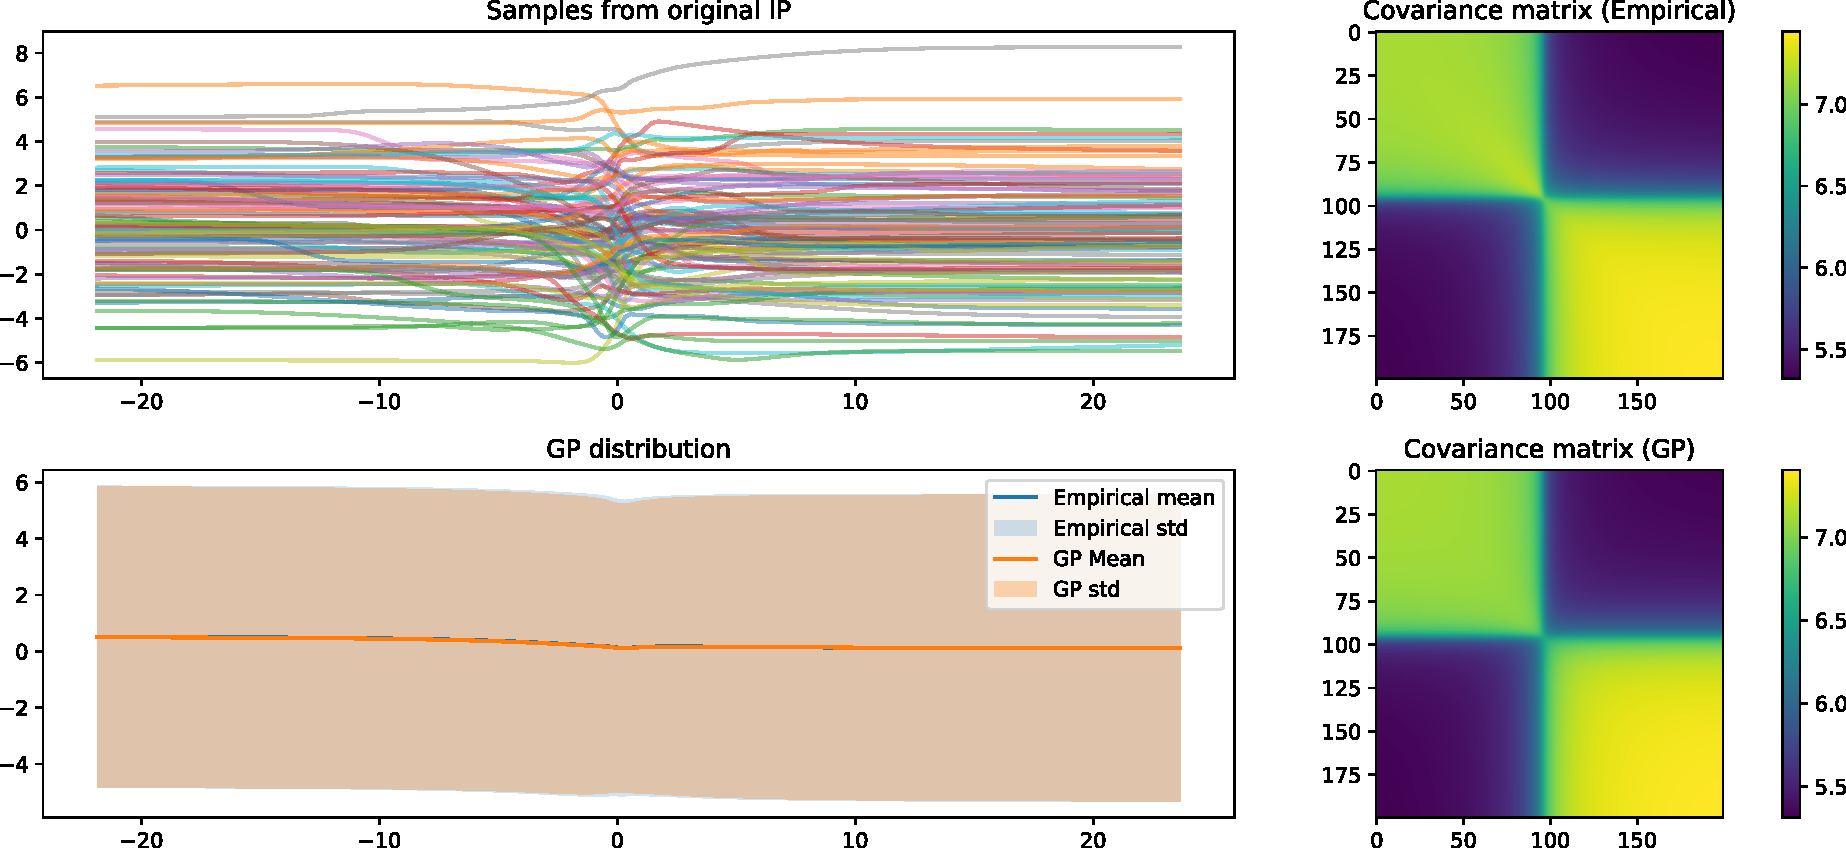
\includegraphics[width=0.95\textwidth]{imgs/GP_cov.pdf}
        \end{center}
    \end{frame}

    \begin{frame}
        \begin{center}
            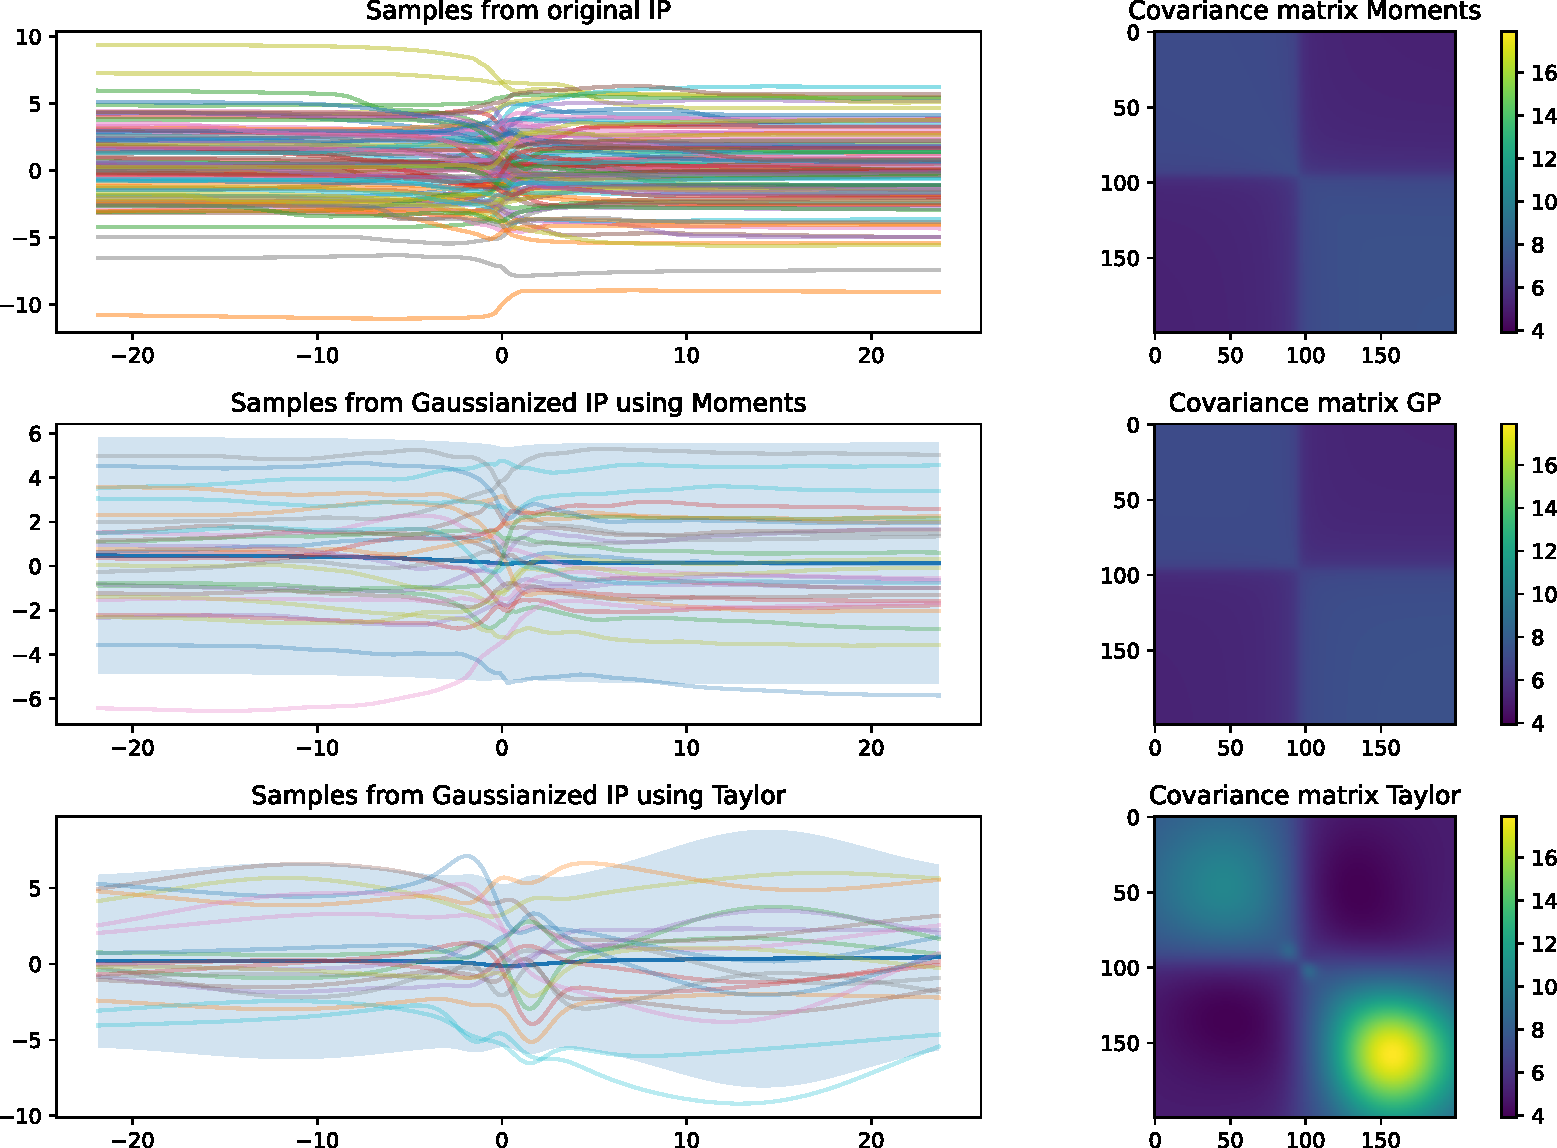
\includegraphics[width=0.8\textwidth]{imgs/GP_taylor.pdf}
        \end{center}
    \end{frame}

    \begin{frame}{Exact posterior distributions}
        We are considering three main models based on the stochastic function 
        \[
            f(\mathbf x) = \frac{1}{\sqrt{H}}\bm w_2^T \phi(\bm w_1^T \mathbf x + \bm b_1) + b_2\,.
        \]
        \begin{enumerate}
            \item The \textbf{exact GP} of the stochastic function.
            \item A GP where the mean and covariance are estimated using \textbf{samples} from the stochastic function.
            \item A GP where the mean and covariance are the ones obtained from the \textbf{Taylor} approximation.
        \end{enumerate}

        We are testing these three methods on a toy 1-D dataset where the exact GP posteriors can be computed.
    \end{frame}

    \begin{frame}
        \begin{center}
        \begin{tabular}{ c c }
         Theoretical GP & GP Samples \\ 
         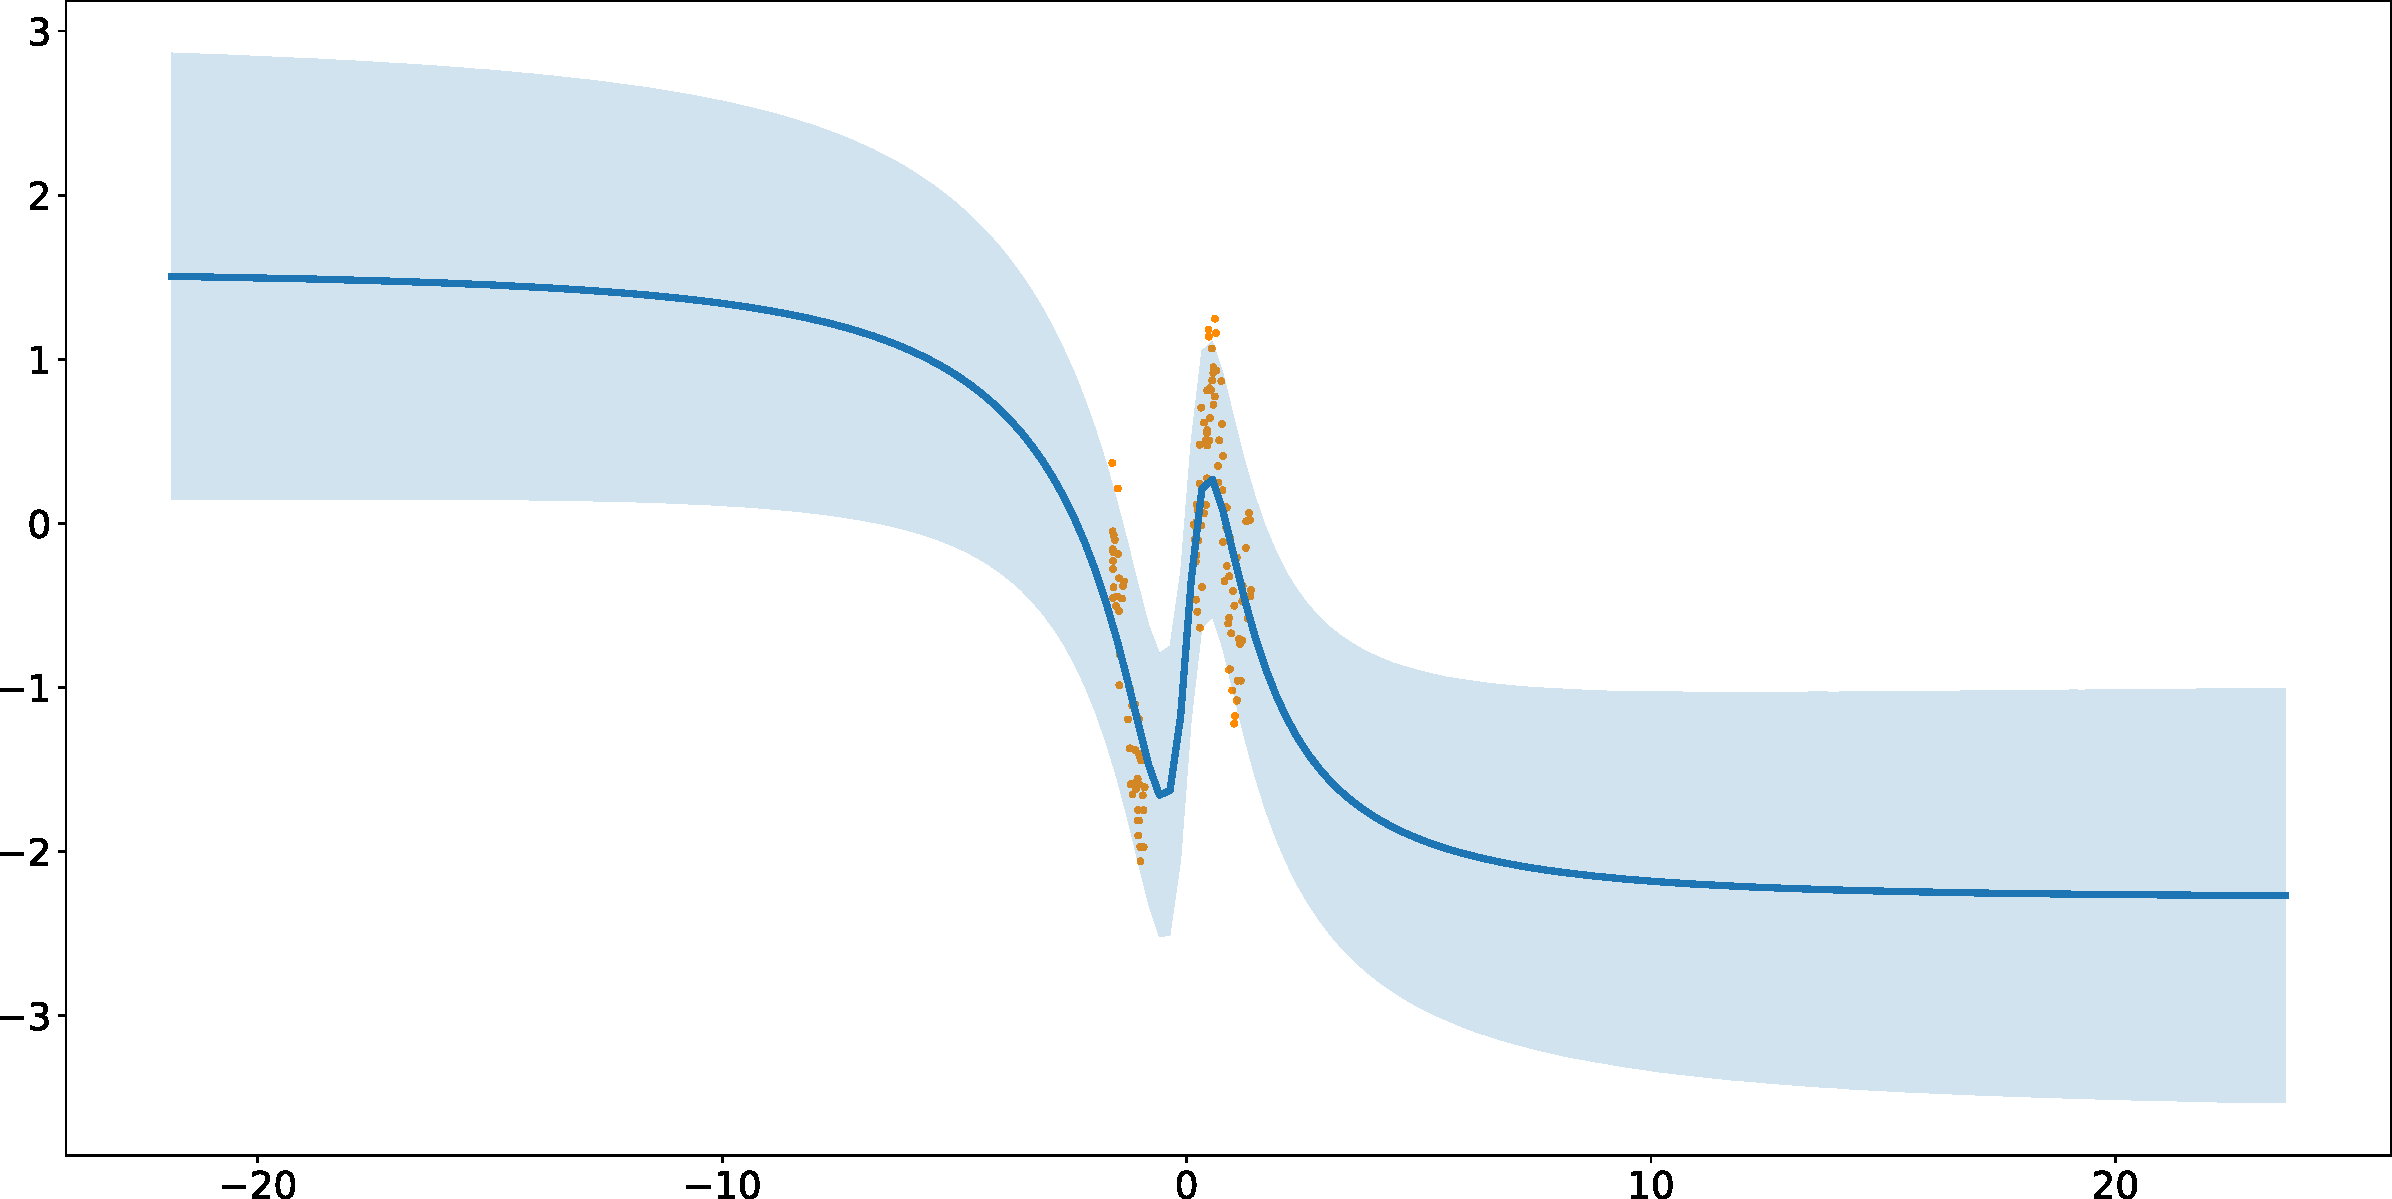
\includegraphics[width=0.49\textwidth]{imgs/Exact_GP.pdf} & 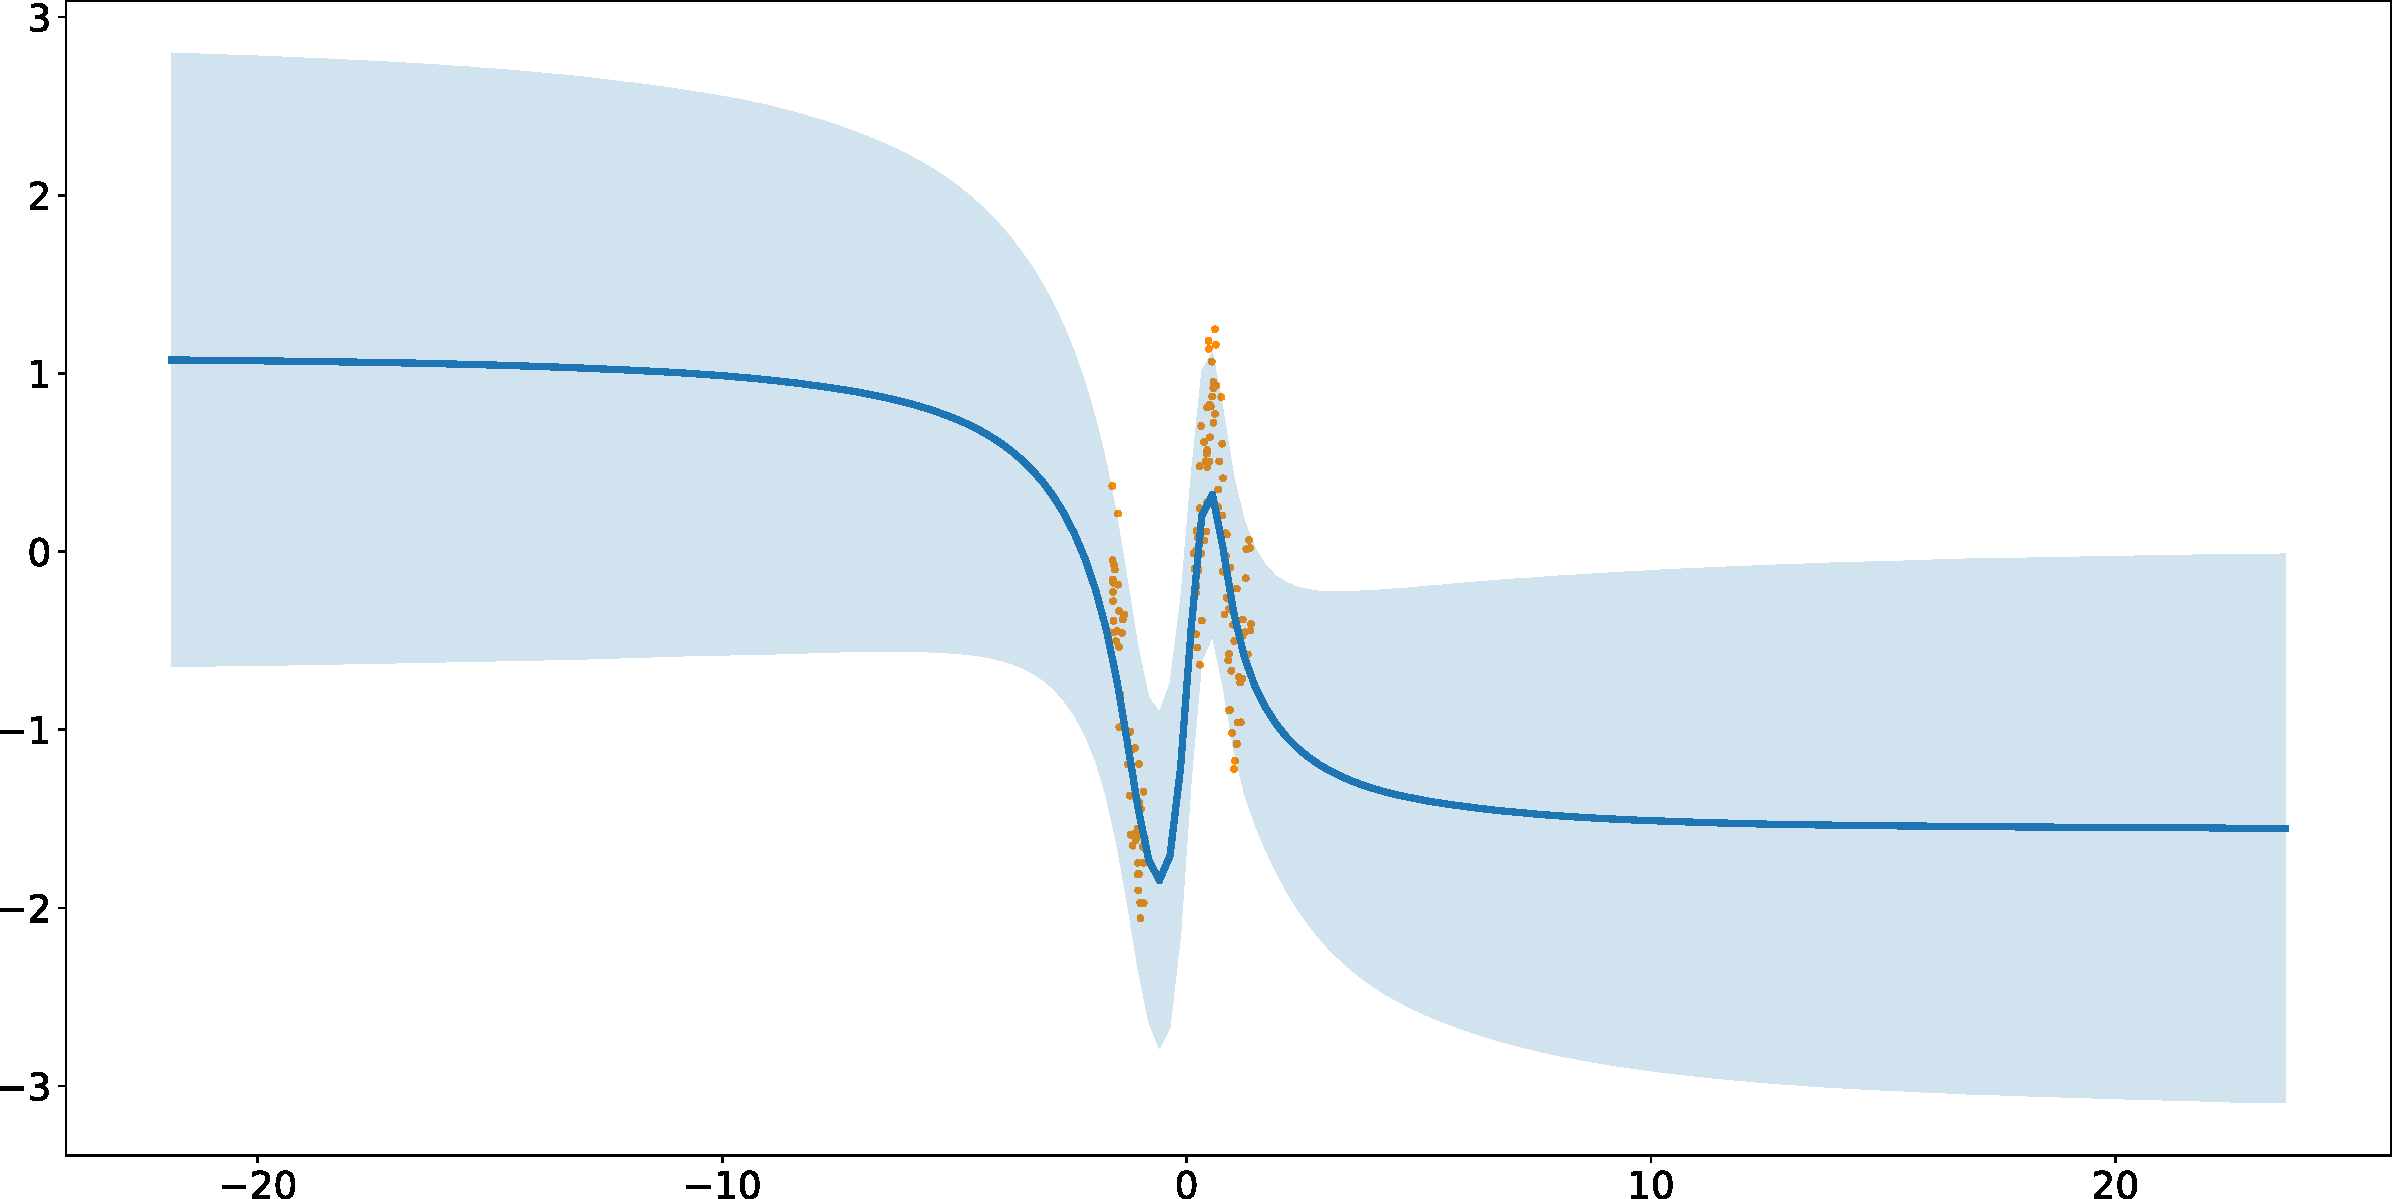
\includegraphics[width=0.49\textwidth]{imgs/Exact_GP_moments.pdf}\\  
        \end{tabular}
        \end{center}
        \begin{center}
        \begin{tabular}{ c}
         GP Taylor \\ 
         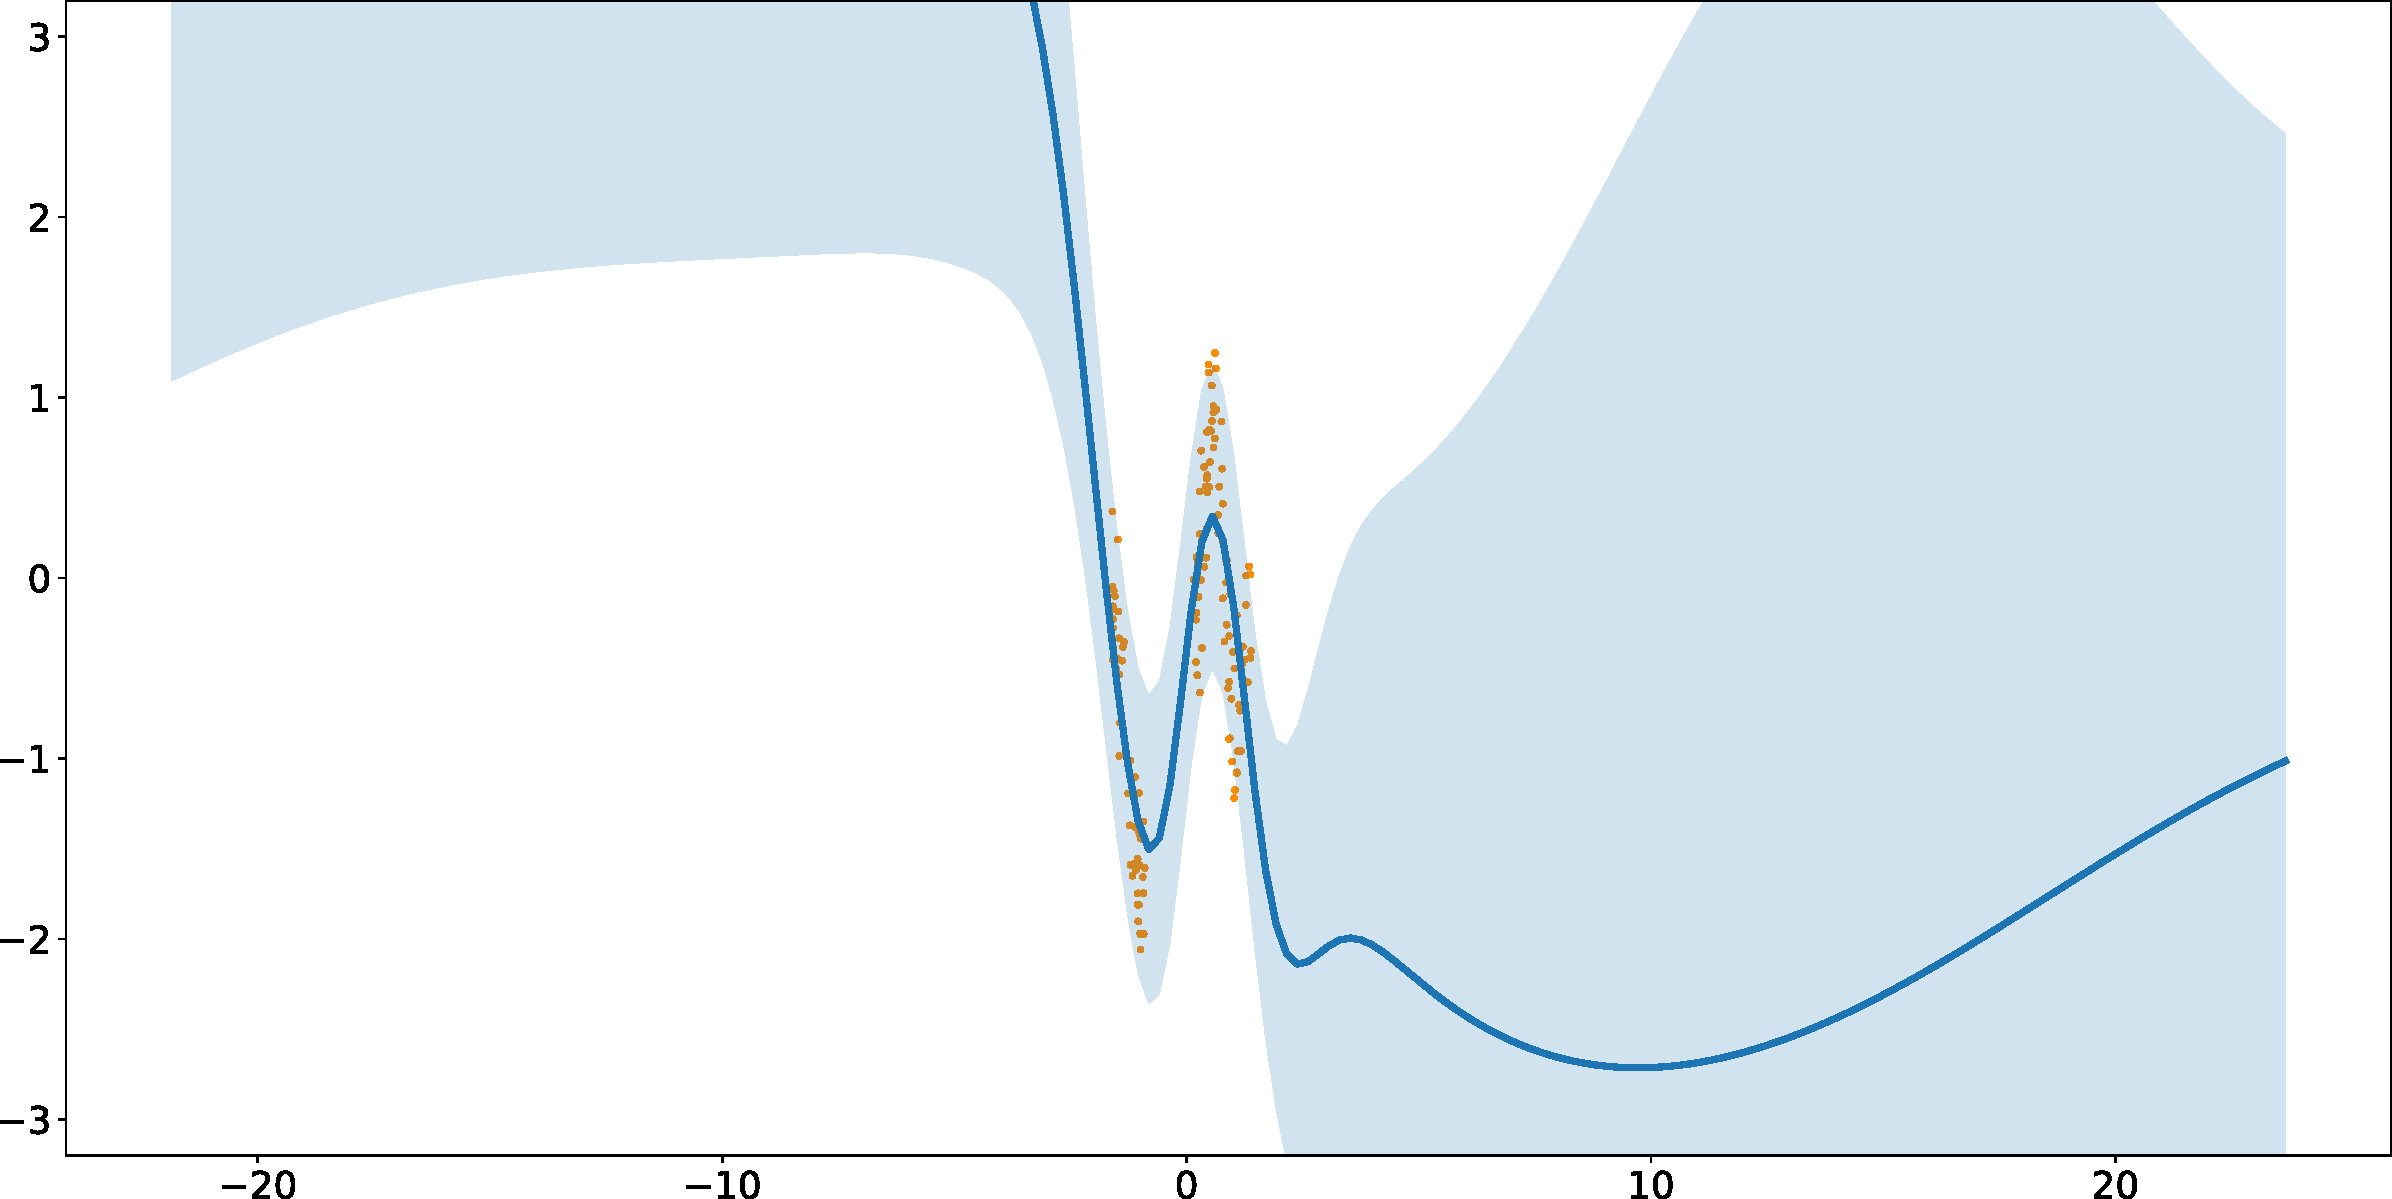
\includegraphics[width=0.49\textwidth]{imgs/Exact_GP_taylor.pdf}\\  
        \end{tabular}
        \end{center}
    \end{frame}


\section{Conclusions}
\begin{frame}{Conclusions}
    \begin{itemize}[<+->]
    \item The Taylor approximation of order 1 is \textbf{not really close} to the exact distribution in the tested cases.
    \item \textbf{However}, preliminary results show that the predictive distribution close to the known points \textbf{is good enough} to encourage more research and testing.
    \item If the Taylor approximation results usable in practise, the proposed method would \textbf{avoid some of the problems of other function-space approaches}.
    \item The family of priors on which the Taylor approximation is good enough needs to be studied.
    \end{itemize}
\end{frame}

\begin{frame}[standout]
  Thank you for your attention
\end{frame}

\end{document}